\documentclass[mstat,12pt]{unswthesis}
\linespread{1}
\usepackage{amsfonts}
\usepackage{amssymb}
\usepackage{amsthm}
\usepackage{latexsym,amsmath}
\usepackage{graphicx}
\usepackage{afterpage}
\renewcommand{\baselinestretch}{1.5}
% \newcommand{\R}{\mathbb{R}}
% \newcommand{\Q}{\mathbb{Q}}
% \newcommand{\C}{\mathbb{C}}
% \newcommand{\N}{\mathbb{N}}
% \newcommand{\F}{\mathbb{F}}
% \newcommand{\PP}{\mathbb{P}}
% \newcommand{\T}{\mathbb{T}}
% \newcommand{\Z}{\mathbb{Z}}
% \newcommand{\B}{\mathfrak{B}}
% \newcommand{\BB}{\mathcal{B}}
% \newcommand{\M}{\mathfrak{M}}
% \newcommand{\X}{\mathfrak{X}}
% \newcommand{\Y}{\mathfrak{Y}}
% \newcommand{\CC}{\mathcal{C}}
% \newcommand{\E}{\mathbb{E}}
% \newcommand{\cP}{\mathcal{P}}
% \newcommand{\cS}{\mathcal{S}}
% \newcommand{\A}{\mathcal{A}}
% \newcommand{\ZZ}{\mathcal{Z}}
% %%%%%%%%%%%%%%%%%%%%%%%%%%%%%%%%%%%%%%%%%%%%%%%%%%%%%%%%%%%%%%%%%%%%%
% %
% % The following are much more esoteric commands that I have left in
% % so that this file still processes. Use or delete as you see fit
% %
% \newcommand{\bv}[1]{\mbox{BV($#1$)}}
% \newcommand{\comb}[2]{\left(\!\!\!\begin{array}{c}#1\\#2\end{array}\!\!\!\right)
% }
% \newcommand{\Lat}{{\rm Lat}}
% \newcommand{\var}{\mathop{\rm var}}
% \newcommand{\Pt}{{\mathcal P}}
% \def\tr(#1){{\rm trace}(#1)}
% \def\Exp(#1){{\mathbb E}(#1)}
% \def\Exps(#1){{\mathbb E}\sparen(#1)}
% \newcommand{\floor}[1]{\left\lfloor #1 \right\rfloor}
% \newcommand{\ceil}[1]{\left\lceil #1 \right\rceil}
% \newcommand{\hatt}[1]{\widehat #1}
% \newcommand{\modeq}[3]{#1 \equiv #2 \,(\text{mod}\, #3)}
% \newcommand{\rmod}{\,\mathrm{mod}\,}
% \newcommand{\p}{\hphantom{+}}
% \newcommand{\vect}[1]{\mbox{\boldmath $ #1 $}}
% \newcommand{\reff}[2]{\ref{#1}.\ref{#2}}
% \newcommand{\psum}[2]{\sum_{#1}^{#2}\!\!\!'\,\,}
% \newcommand{\bin}[2]{\left( \begin{array}{@{}c@{}}
% 				#1 \\ #2
% 			\end{array}\right)	}
% %
% %  Macros - some of these are in plain TeX (gasp!)
% %
% \newcommand{\be}{($\beta$)}
% \newcommand{\eqp}{\mathrel{{=}_p}}
% \newcommand{\ltp}{\mathrel{{\prec}_p}}
% \newcommand{\lep}{\mathrel{{\preceq}_p}}
% \def\brack#1{\left \{ #1 \right \}}
% \def\bul{$\bullet$\ }
% \def\cl{{\rm cl}}
% \let\del=\partial
% \def\enditem{\par\smallskip\noindent}
% \def\implies{\Rightarrow}
% \def\inpr#1,#2{\t \hbox{\langle #1 , #2 \rangle} \t}
% \def\ip<#1,#2>{\langle #1,#2 \rangle}
% \def\lp{\ell^p}
% \def\maxb#1{\max \brack{#1}}
% \def\minb#1{\min \brack{#1}}
% \def\mod#1{\left \vert #1 \right \vert}
% \def\norm#1{\left \Vert #1 \right \Vert}
% \def\paren(#1){\left( #1 \right)}
% \def\qed{\hfill \hbox{$\Box$} \smallskip}
% \def\sbrack#1{\Bigl \{ #1 \Bigr \} }
% \def\ssbrack#1{ \{ #1 \} }
% \def\smod#1{\Bigl \vert #1 \Bigr \vert}
% \def\smmod#1{\bigl \vert #1 \bigr \vert}
% \def\ssmod#1{\vert #1 \vert}
% \def\sspmod#1{\vert\, #1 \, \vert}
% \def\snorm#1{\Bigl \Vert #1 \Bigr \Vert}
% \def\ssnorm#1{\Vert #1 \Vert}
% \def\sparen(#1){\Bigl ( #1 \Bigr )}
% \newcommand\blankpage{%
%     \null
%     \thispagestyle{empty}%
%     \addtocounter{page}{-1}%
%     \newpage}
% \newtheorem{theorem}{Theorem}[section]
% \newtheorem{lemma}[theorem]{Lemma}
% \newtheorem{proposition}[theorem]{Proposition}
% \newtheorem{corollary}[theorem]{Corollary}
% \newtheorem{conjecture}[theorem]{Conjecture}
% \newtheorem{definition}[theorem]{Definition}
% \newtheorem{example}[theorem]{Example}
% \newtheorem{remark}[theorem]{Remark}
% \newtheorem{question}[theorem]{Question}
% \newtheorem{notation}[theorem]{Notation}
% \numberwithin{equation}{section}
\hyphenation{Mar-cin-kie-wicz Rade-macher}


%%%%%%%%%%%%%%%%%%%%%%%%%%%%%%%%%%%%%%%%%%%%%%%%%%%%%%%%%%%%%%%%%
%
%  And now the document begins
%  The \beforepreface and \afterpreface commands puts the
%  contents page etc in
%
%%%%%%%%%%%%%%%%%%%%%%%%%%%%%%%%%%%%%%%%%%%%%%%%%%%%%%%%%%%%%%%%%%
\title{Layerwise Inference for Dirichlet Belief Networks}

\authornameonly{Huiqiang Zhong}

\author{\Authornameonly\\{\bigskip}Supervisor: Dr. Xuhui Fan}

\copyrightfalse
\figurespagefalse
\tablespagefalse

\begin{document}

\beforepreface

\afterpage{\blankpage}

% plagiarism
\prefacesection{Plagiarism statement}

\vskip 10pc \noindent I declare that this thesis is my
own work, except where acknowledged, and has not been submitted for
academic credit elsewhere.

\vskip 2pc  \noindent I acknowledge that the assessor of this
thesis may, for the purpose of assessing it:
\begin{itemize}
\item Reproduce it and provide a copy to another member of the University; and/or,
\item Communicate a copy of it to a plagiarism checking service (which may then retain a copy of it on its database for the purpose of future plagiarism checking).
\end{itemize}

\vskip 2pc \noindent I certify that I have read and understood the University Rules in
respect of Student Academic Misconduct, and am aware of any potential plagiarism penalties which may
apply.\vspace{24pt}

\vskip 2pc \noindent By signing
this declaration I am
agreeing to the statements and conditions above.
\vskip 2pc \noindent
Signed: \rule{7cm}{0.25pt} \hfill Date: \rule{4cm}{0.25pt} \newline
\vskip 1pc

\afterpage{\blankpage}

% Abstract
\prefacesection{Abstract}
\begin{enumerate}

  Topic model,especially latent Dirichlet allocation(LDA),has aroused grea research interest in the past two decades which is a useful tools for document classification.The LDA model assume that word of doucment is determined by the topic of document and topic-word matrix.Some multi-layer generative process on word distribution on have been proposed to improve LDA.However it suffer from information decay and complicate samping method. Here we present a Dirichlet-Belief Networks to address problems above. By inserting auxiliary Poisson ran-dom variables into the layerwise connections and appropriate design, we can inference latent parameter in an efficient way.As an Bayesian generatice model,it is more interpretability and gibbs sampling can be used in training model.

  % \begin{itemize}
  %   \item domain of research,purpose
  %   \item research method
  %   \item result of test
  %   \item mainpoint.breaking_point
  %   \item The problem I am trying to solve in this paper is
  %   \item The approach I adopt to solve the problem is
  %   \item The results obtained in this research include
  %   \item impacts of our obtained results are ...
  % \end{itemize}




\afterpage{\blankpage}
\afterpreface

%%%%%%%%%%%%%%%%%%%%%%%%%%%%%%%%%%%%%%%%%%%%%%%%%%%%%%%%%%%%%%%%%%
%
% Now we can start on the first chapter
% Within chapters we have sections, subsections and so forth
%
%%%%%%%%%%%%%%%%%%%%%%%%%%%%%%%%%%%%%%%%%%%%%%%%%%%%%%%%%%%%%%%%%%
%%%%%%%%%%%%%%%%%%%%%%%%%%%%%%%%%%%%%%%%%    Chapter 1
\afterpage{\blankpage}

\chapter{Introduction}\label{s-intro}

\section{Background and Importance}
With the development of technology and alomost all information is digitized, we are more and more likely to be overwhelmed by a large amount of information, and it is difficult to find an effective way to find, organize and understand a large amount of information{\cite{intro-back}}.Then, how to effectively obtain better information and how to automatically classify vast amounts of text data, organization and management become more challenging. Therefore, in the face of these problems and needs, the use of computers for language information processing has been extensively studied. As a research hotspot in the field of natural language processing, automatic text classification technology has been rapidly developed and widely used.


Such data is sparse and discrete date which is hard for computer to process.The bag of words models are proposed for samplifying representation in natural language processing.This model can convert a sentence into a vector representation, which is a relatively straightforward method. It does not consider the order of words in the sentence, only considers the number of occurrences of words in the vocabulary in this sentence so that it will miss the relationshaip between each individual vocabulary and induces huge prolem of dimensional disaster. However it still a popular way in representing document.

After representing document by matrix,scientists hope to construct a generative model to
Imitate document writing. It reduces a complex precudure into some probabilistic steps and specify a sample  distribution for the topic of  document\cite{find}. We will introduce  a very well-known method in natural language processing - Latent Dirichlet Allocation(LDA) which can extract  abstract "themes"  from a series of documents through the mechanism of generating models.


This model assumes the implicit mechanism of published documents written by humans: each document is composed of a few topics, and each topic can be composed of a few important words description. In other words, When writing an article, we will first decide the topics related to our document, then each word we write in text is closely related to these topics.Let's follow the generative process of LDA step by step:
\begin{itemize}
  \item For each document, we extract a theme from the theme distribution.
  \item Extracting a word from the word distribution corresponding to the above-mentioned theme.
  \item Repeat the above process until each word in the document is traversed.
\end{itemize}

This generative process is mainly compose of two distributions-the topic distribution of each docuemnt and the word distribution of each topic.In LDA, the topic distribution and word distribution are uncertain. The authors of LDA adopt the Bayesian idea that they should obey a distribution. The topic distribution and word distribution are subject to  polynomial distributions,so the topic distribution and word distribution use Dirichlet distribution as their conjugate prior distribution because the polynomial distribution and Dirichlet distribution is a conjugate structure.

As mentioned above,one commonly-used prior for topic distribution and word distribution is diriclet distribution and recently lots of distributions have been imposed on topic distribtion.For example,The correlation topic model(CTM)\cite{corr},which exhibits the correlation of topic by introducing logistic noremal distribution.It allows each document to show different topics with different proportions and capture the relationship in groud data.Besides,there are hierarchical document representation based on dirichlet process and Boltzmann machines and neural network.\cite{zhao}.


% Mention of previous work on the subject
% Statemeng of the importance of the subject

% 引言部分的第一段需要给出研究领域的大背景及其重要性所在。这个大背景勾勒出该领域科研成果从古至今的一个走向或者趋势 (what is known),为接下来本论文课题的发展生长提供温床。这部分内容的展开一定要引用该领域前人、大牛的经典文献或者奠基性著作,体现你对于该学科的一个总体把握是全面且客观的。那如何从这个大背景引入到论文的课题呢?当我们从该学术领域的大趋势逐渐缩小范围时,只需把其中
?
% 摆出该研究领域的一个概况之后,就要顺理成章地指出哪些是我们还未涉及的领域(或是没有研究透彻的问题)。当然这样的问题有千千万万,此处不能全部罗列,必要要对应着你的论文课题来谈。直白地说,就是你论文课题研究的什么,此处就针对性地写“这个课题尚未被太多科研者涉足”云云。

\section{topic of research paper}
Announce the research topic/question being addressed in research paper

% 既然研究空白已近在眼前,那么对应的研究课题便要紧随其后。接下来就是你理直气壮陈述该论文主题的时刻,此时需要注意与研究空白的呼应,即在摆出课题是什么的基础之上更近一层,简要分析这个课题是

\section{Highlight the approach and principal finding}

DEscrition of your paper approach and why you chose it

brief summary of your major findings

\section{Organization of this paper}

%%%%%%%%%%%%%%%%%%%%%%%%%%%%%%%%%%%%%%%%%    Chapter 2
\chapter{Basic language}
%%%%%%%%%%%%%%%%%%%%%%%%%%%%%%%%%%%%%
In this chapter we outline the basic background of Latent Dirichlet Allocation
. We begin by reviswing the Bayesian Theorem
associated with functional analysis in LDA. Then some common statistic distributions
 will be introduced which are used in inferencing posterior distribution and latend parameters.Sampling techniques such as Gibbs Sampling which is frequently used to obtain results of model will be listed in last subsection.

\section{Bayesian Theorem}\label{Banach Spaces}
We can never be completely sure of this world, because it is a constantly changing being, and change is the essence of reality. However, what we can do is, as expressed by this theorem, as we obtain more and more data or evidence, our knowledge of reality has been updated and improved
\begin{eqnarray*}
P(A|B) &=& \frac{P(A,B)}{P(B)} \\
& = &\frac{P(B|A)*P(A)}{P(B)} \\
\end{eqnarray*}
\begin{itemize}
  \item $P(A | B)$ is the conditional probability of A after the occurrence of B is known, and is also excluded from the posterior probability of A due to the value obtained from B, indicating the confidence that event A will occur after event B occurs.

  \item $P(A)$ is the a priori probability or edge probability of A, and represents the confidence that event A occurs.

  \item $P(B|A)$ is the conditional probability of B after the occurrence of A. It is also called the posterior probability of B because of the value obtained from A, and is also considered as a likelihood function.

  \item $P(B)$ is the prior probability or edge probability of B, which is called a standardized constant.

  \item $P(B | A) P(B)$ is called the standard likelihood ratio (there are many names, and no unified standard name is found), which indicates the degree of support provided by event B for the occurrence of event A.
\end{itemize}
\subsection{Prior Probability}

A priori probability refers to an event that has not yet occurred, and an estimate of the probability of the event occurring, describing a variable in the absence of something.Prior information comes from experience and historical data

\subsection{Likelihood Probability}
\begin{itemize}
  \item If the "probability function" P(B|A)/P(B)>1, it means that the "prior probability" is enhanced and the probability of the occurrence of event A becomes greater;
  \item If "probability function" = 1, it means that event B does not help to determine the possibility of event A;
  \item If the "probability function" <1, it means that the "prior probability" is weakened, and the probability of event A becomes smaller.
\end{itemize}
\subsection{Posterior probability}
The posterior probability refers to the probability that the cause of the event is caused by a factor under the condition that the event has occurred. It is the conditional probability after considering an event.

\subsection{conjugate prior}
The posterior probability distribution function has the same form as the prior probability distribution function
If the prior distribution and the likelihood function can make the prior distribution and the posterior distribution (posterior distributions) have the same form, then the prior distribution and the likelihood function are said to be conjugate. Therefore, conjugate refers to the prior probability distribution and likelihood function. If the posterior probability p(θ|x) and the gas prior probability p(θ) of a random variable Θ belong to the same distribution cluster, then p(θ|x) and p(θ) are called conjugate distributions, and , Also called p(θ) is the conjugate prior of the likelihood function p(x|θ).


The conjugate prior and posterior have the same form. This can easily form an iteration in the calculation process. According to the new observation data, the original posterior probability becomes a new prior probability, and then a new posterior probability is updated. The parameters of this posterior probability are more accurate. . This process greatly simplifies Bayesian analysis

\section{Basic distribution}

\subsection{Beta distribution}
The beta distribution can represent the probability distribution of a probability. When you don't know the specific probability of a thing, it can be called the probability of the occurrence of all probabilities

Definition The Beta Function,For each positive $\alpha$ and $\beta$.define:
$$P(x|\alpha,\beta) = \frac{1}{B(\alpha,\beta)}x^{\alpha-1}(1-x)^{\beta-1} $$
%
% The function B is called beta function.
$$B(\alpha,\beta) = \frac{\Gamma(\alpha)  \Gamma(\beta)}{\Gamma{\alpha+\beta}}$$

For example,carry out $N$ times of Bernoulli test, the probability of success of the test p is subject to an a priori probability density distribution $Beta(\alpha,\beta)$ , the test result appears $K$ times of success of the test, the posterior probability density distribution of the probability p of the test success is $Beta(\alpha + K,\beta+N-K)$.Prove:

Prior distribution:
\[
  f(p|\alpha,\beta) &=& \frac{\Gamma(\alpha)  \Gamma(\beta)}{\Gamma{\alpha+\beta}}x^{\alpha-1}(1-x)^{\beta-1} \
\]
Likelihood Function:
\[
  f(n_1,n_2,\ndot,N|p) = p^{K}(1-p)^{N-K}
\]
Posterior distribution:
\begin{eqnarray*}
  f(p|n_1,n_2,..N,\alpha,\beta) &=& \frac{f(n_1,n_2,\ndot,N|p)f(p|\alpha,\beta)}
  {f(n1,n2,...N,\alpha,\beta)}
\end{eqnarray*}

Given that:
\begin{eqnarray*}
  f(n1,n2,...N,\alpha,\beta) &=& \int_p f(n_1,n_2,\ndot,N|p)f(p|\alpha,\beta) \\
  & = &\frac{1}{B(\alpha,\beta)} \int_p p^{\alpha+K-1}(1-p)^{\beta+N-K-1} \\
  &=&  \frac{B(\alpha+k,\beta+N-K)}{B(\alpha,\beta)}
\end{eqnarray*}
\begin{eqnarray*}
  f(n_1,n_2,\ndot,N|p)f(p|\alpha,\beta) &=& \frac{1}{B(\alpha,\beta)}x^{\alpha-1}(1-x)^{\beta-1} * \frac{f(n_1,n_2,\ndot,N|p)f(p|\alpha,\beta)}
  {f(n1,n2,...N,\alpha,\beta)} \\
  &=& \frac{1}{B(\alpha,\beta)}p^{\alpha+K-1}(1-p)^{\beta+N-K-1}
\end{eqnarray*}

So that:
\begin{eqnarray*}
  f(p|n_1,n_2,..N,\alpha,\beta) &=& \frac{1}{\alpha+K-1}(1-p)^{\beta+N-K-1}p^{\alpha+K-1}(1-p)^{\beta+N-K-1} \\
  &=& Beta(\alpha + K,\beta+N-K)
\end{eqnarray*}


\subsection{Dirichlet distribution}
Dirichlet distribution is a generalization of the beta distribution in high dimensions
\subsection{Poisson and Multinomal distribution}
\subsection{conclusion}
Taking a coin toss as an example, after you get a coin, normally the probability of a uniform coin appearing on both sides should be the same, both 0.5, but you are not sure about the material and weight distribution, you need to judge its Is it really evenly distributed

\section{Markov Chain Monte Carlo and Gibbs Sampling}\label{bases}

\subsection{Monte Carlo Method}
The Monte Carlo method is a calculation method. The core is to understand a event through a large number of random samples, and then get the result by smaples.

It is a very powerful and flexible method, and quite easy to understand and implement. For many problems, it is often the simplest calculation method, and sometimes even the only feasible method.
As a random sampling method, Markov Chain Monte Carlo has a wide range of applications in the fields of machine learning, deep learning, and natural language processing. It is also the basis of many complex algorithms.

The early Monte Carlo methods were designed to solve some summation or integration problems that are not very easy to solve. Such as:
\[
Y = \int_a^b f(x)

\]

The answer can be deducted by Newton-Leibniz formula if the function is simple enough. However,
in most cases, it is difficult to find the primitive function of $f(x)$. So that people introduce Monte Carlo method  which can get the approximation of $Y$ by large number of samples.

People can sample $n$ values ​​in the interval $[a,b]$: $x_1,\dots,x_n$, and use their average values ​​to represent all $f(x)$ values ​​in the $[a,b]$ interval. So our approximate solution to the integral above is:
\[
  Y = \frac{b-a}{n}\sum^n f(x_i)
\]

The above method has an implicit assumption that the distribution of $x$ follows a uniform distribution from a to b, but the actual situation is that it will subject to  various types of distribution. Improving the method as follows:
\begin{eqnarray*}
Y &=& \int_a^b f(x) \\
  &=& \int_a^b \frac{f(x)}{p(x)}p(x) \\
  &=& \frac{1}{n} \sum^n \frac{f(x_i)}{p(x_i)}\\
\end{eqnarray*}

The main question now turns to how to find the distribution of $x$

\subsection{Sampling Method}
The key to the Monte Carlo method is to get the probability distribution of $x$. If the probability distribution of $x$ is found,$n$ sample sets based on this probability distribution can be sampled and it can be brought into the Monte Carlo integration formula to solve problem.

For the common uniform distribution $\mathcal U (0,1)$, it is very easy to get samples, generally through the linear congruential generator that can easily generate between (0,1) Pseudo-random number samples. For other common probability distributions, whether they are discrete distributions or continuous distributions, their samples can be infered by sample conversion of uniform distribution.

Assuming that $x$  which is a continuous random variable, is subject to a random distribution $f(x)$ and its cumulative distribution function is $F(X)$. Besides, assuming that $Y = F(X)$ is subject to $\mathcal U (0,1)$ and $F^{-1}(Y)$ have same distribution with $X$. For example:

PDF of Expoential distribution:
\[
  f(x) = \lambda e^{\lambda*x}
\]
CDF of Expoential distribution:
\[
  F(x) = 1- exp^{\lambda*x}
\]
Inverse sampling inference:

\begin{eqnarray*}
u & \sim & Uniform(0,1) \\
F(F^{-1}(Y)) &=& 1- exp^{\lambda*F^{-1}(Y)} = u \\
F^{-1}(Y) &=&-\frac{\log(1-u)}{\lambda}
\end{eqnarray*}

But many times, the probability distribution is not a common distribution, which means that it is hard to get a sample set of these unusual probability distributions. So,Reject-Sampling method is proposed.

\begin{figure}
  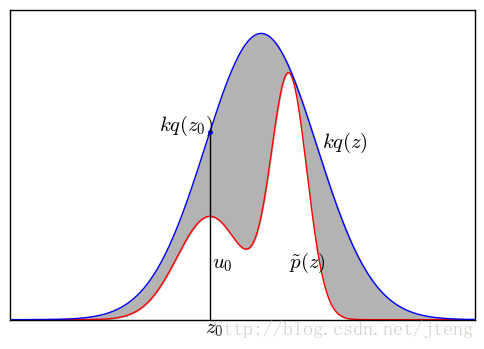
\includegraphics[width=\linewidth]{reject.png}
  \caption{Reject-Sampling Method}
  \label{fig:boat1}
\end{figure}

The basic idea of Reject-Sampling \cite{samp} is to cover the smaller probability distribution with a larger probability distribution. This larger probability distribution $q(x)$ called proposal distribution  and  usually it is a standard distribution such as Uniform distribution, Gaussian distribution, which makes it easier to sample. Then there is a constant $k$ which make $k*q(x) \leq p(x)$.

In each sample process:

\begin{itemize}
  \item Sample a value $x$ from proposal distribution $q(x)$
  \item Get a sample $\mu_0$ from Uniform distribution $[0,k*q(\mu_0)]$.
  \item If $\mu_0 < p(x)$ ,we retain the value otherwise we discard this value. The sampled set is an approximate sample of  distribution.
\end{itemize}

Some cases can be solved  by Reject-Sampling when the probability distribution is not common. However,in the case of high dimensions, Rejection Sampling will encounter two problems. The first is that the proposal  distribution $q$ is difficult to find, and the second is that it is difficult to determine a reasonable value of $k$. These two problems will lead to a high rejection rate and an increase in useless calculations.


\subsection{Markov Chain}
Markov Chain is a random process from state to state in the state space. This process introduce no memory attribute: the probability distribution of the next state can only be determined by the current state, and the events before it in the time series have nothing to do with it. This special type of no memory is called the Markov attribute and as a powerful statistical models Markov chains have many applications in the real world.

At each step of the Markov chain, the system can change from one state to another according to the probability distribution and it also can maintain the current state when it reachs stable state. The change of state is called transition, and the probability associated with different state changes is called transition probability.

In order to obtain a theoretical result, let's look at a smaller example which will facilitate our  calculation demonstration later. Assuming that in a region, people either live in the city or live in the countryside. The matrix below tells us the transition matrix of population migration. For example, the number of the first column  and first row indicates that 90 \% of the population currently living in cities will choose to  live in cities next year and 80 \% of people who live in country will continue to stay in country.
$$
H_x={
\left[ \begin{array}{ccc}
0.9 & 0.1 \\
0.2 & 0.8\\
\end{array}
\right ]}
$$

People assume that nowadays half of the people live in the city and the other half are in the countryside. As a simple start, researchers try to estimate that how much of people will live in city after two years. Analysis shows that 90 \% of people  who currently living in the city will continue to  live in the city after 1 year, and 10\% of people will move to the country. Then another year passed, and 10 \% of those who chose to stay in the city last year moved to the countryside. And 80 \% of those who moved to the village last year will choose to stay in the village. This analysis process is shown  below.
One year later:

$$
H_x=  {
\left[ \begin{array}{ccc}
0.5  & 0.5 \\
\end{array}
\right ]}
\times{
\left[ \begin{array}{ccc}
0.9 & 0.1 \\
0.2 & 0.8\\
\end{array}
\right ]}
=
{
\left[ \begin{array}{ccc}
0.55 & 0.45 \\
\end{array}
\right ]}
$$

One year later:

$$
H_x=  {
\left[ \begin{array}{ccc}
0.55 & 0.45 \\
\end{array}
\right ]}
\times{
\left[ \begin{array}{ccc}
0.9 & 0.1 \\
0.2 & 0.8\\
\end{array}
\right ]}
=
{
\left[ \begin{array}{ccc}
0.585 & 0.415 \\
\end{array}
\right ]}
$$

In fact,it is easy to find that the calculation process above is to do the square of the matrix. As shown in the formula above,on this basis, we can also continue to calculate the situation after $n$ years, that is, the result of calculating the self-multiplication of matrix $A$ n time

The algorithm is as follows:
\begin{itemize}
  \item Enter the Markov chain state transition matrix, set the state transition times threshold,the required number of samples.
  \item Samplfrom any simple probability distribution to get the initial state value.
  \item sample  from the conditional probability distribution and The sample set is the corresponding sample set that meets our stationary distribution.
\end{itemize}

Given the Markov chain state transition matrix corresponding to the stationary distribution of the samples needed to sample, then people can use the Markov chain sampling to obtain the sample set, and then execute Monte Carlo simulation.

But an important question is, given a random distribution at will, how to get the Markov chain state transition matrix $P$ corresponding to it?

\subsection{MCMC  and M-H Sampling}
Mostly, target stationary distribution $\pi(x)$ and a certain Markov chain state transition matrix $Q$ does not satisfy the detailed balance condition:
\[
  \pi(i)Q(i,j) \neq \pi(j)Q(j,i)
\]


a parameter $\alpha(i,j)$ is introduced so that the above formula can take the equal sign.
\[
  \pi(i)Q(i,j)\alpha(i,j) = \pi(j)Q(j,i)\alpha(j,i)
\]

The $\alpha$ can be deducted by symmetry:
\begin{eqnarray*}
\alpha(i,j) &=& \pi(j)Q(j,i)\\
\alpha(j,i) &=& \pi(i)Q(i,j)
\end{eqnarray*}


$\alpha$ is generally called acceptance rate, and the value is between $[0 \sim 1]$, which can be understood as a probability value. This is much like accept-reject sampling, where a common distribution is obtained through a certain acceptance-rejection probability. A common Markov chain with state transition matrix $Q$  can obtain the target sets through a certain acceptance-rejection probability. Obviously the two solutions to the problem are similar\cite{mh}.

MCMC  algorithm is as follows:
\begin{enumerate}
  \item Enter any given Markov chain state transition matrix $Q$, target stable distribution $\pi(x)$, set the threshold of state transition times $n_1$, the number of required samples $n_2$;
  \item Get the initial state value $x_0$ from any simple probability distribution;
  \item For $t$ =0 in $n_1+n_2-1$
    \begin{itemize}
      \item Get the sample value $x_*$ from the conditional probability distribution $Q(x_*|x_0)$.
      \item Sample $U$ from Uniform distribution.
      \item if $u<\pi(x_*)*Q(x_*|x_0)$,then accept $x_*$.
    \end{itemize}
\end{enumerate}


But this sampling algorithm is still more difficult to apply in practice, because in the third step, the accept rate $\alpha$ may be very small, such as 0.1, most of our sampled values ​​are rejected and the sampling efficiency is very low. There is possible that after sampling millions of Markov chains,the result have not yet converged. As a result,the above $n_1$ should be  very large, which is unacceptable.

Metropolis-Hastings sampling also called M-H sampling can solve the problem of low sampling acceptance rate in the previous section.

Expanding both sides of:
\[
  \pi(i)Q(i,j)\alpha(i,j) =  \pi(j)Q(j,i)\alpha(j,i)
\]
At this time the detailed stationary condition is also satisfied. By expanding the equation by $C$ times which can make $c* max(\alpha(i,j)) = 1$ (the maximum expansion of both sides is 1), Metropolis-Hasting sampling significantly improves the acceptance rate.
The transofrmation is:
\[
  \alpha = min(\frac{Q(j,i)\alpha(j,i)}{Q(i,j)\alpha(i,j)},1)
\]

Compare to basic MCMC method, Metropolis Hasting sampling  greatly improves the efficiency of sampling. However, in the era of big data, M-H sampling still faces two major challenges:
\begin{enumerate}

  \item  There are lots of data features and due to the existence of the acceptance rate, the calculation time of M-H sampling required in high dimensions is very considerable, and the algorithm efficiency is very low. At the same time, $ \alpha $ is generally less than 1.  Can it be done without refusing to transfer?

  \item Due to the large feature dimension, it is often difficult to find the joint distribution of each feature dimension of the target, but it is convenient to find the conditional probability distribution between each feature. At this time, is there a  convenient sampling  method in the case of conditional probability distribution between various dimensions?
\end{enumerate}

\subsection{Gibbs Sampling}
Gibbs Sampling Method\cite{bda} is another special MCMC technique used for sampling variales in large dimensions by sampling each variable from its conditional distribution iterative.

Starting from a two-dimensional data distribution, assuming that $\pi(x_1,x_2)$ is a two-dimensional joint data distribution, observe the first two points with the same feature size$A(x_1^{(1)},x_2^{(1)})$ and $B(x_1^{(1)},x_2^{(2))})$.For example:
\[
  \pi(x_1^{(1)},x_2^{(1)})\pi(x_2^{(2)}|x_1^{(1)}) = \pi(x_1^{(1)})\pi(x_2^{(2)}|x_1^{(1)})\pi(x_2^{(1)}|x_1^{(1)})
\]

\[
  \pi(x_1^{(1)},x_2^{(1)})\pi(x_2^{(1)}|x_1^{(1)}) = \pi(x_1^{(1)})\pi(x_2^{(2)}|x_1^{(1)})\pi(x_2^{(1)}|x_1^{(1)})
\]

Since the right sides of the two formulas are equal, we have:
\[
  \pi(x_1^{(1)},x_2^{(1)})\pi(x_2^{(2)}|x_1^{(1)}) =   \pi(x_1^{(1)},x_2^{(1)})\pi(x_2^{(1)}|x_1^{(1)})
\]

Observing the above detail balance formula , it shows that on the straight line of $x_1 = x_1^{(1)}$, if the conditional probability distribution $\pi(x_2|x_1^{(1)})$ is used as the state transition probability of the Markov chain, the transition between any two points meets Detail balance conditions! In the same way, on the straight line of $x_2 = x_2^{(1)}$, if the conditional probability distribution $\pi(x_1|x_2^{(1)})$  is used as the state transition probability of the Markov chain, the transition between any two points also meets the detail balance condition.


With the  transition matrix and conditional probability, a two-dimensional Gibbs sample can be applied to get samples conventiently.
The algorithm is as follows:
\begin{enumerate}
  \item Given stationary distribution $\pi(x_1,x_2)$,Set the threshold value of the number of state transitions $n_1$, the number of required samples $n_2$.
  \item Randomly initialize values $x_1^{(1)}$ and $x_2^{(1)}$.
  \item for t in [0,n1+n2-1]:
      \begin{itemize}
        \item Get sample $x_2^{(t+1)}$ from conditional distribution $p(x_2|x_1^t)$
        \item Get sample $x_1^{(t+1)}$ from conditional distribution $p(x_1|x_2^t)$
      \end{itemize}
\end{enumerate}

%%%%%%%%%%%%%%%%%%%%%%%%%%%%%%%%%%%%%%% 		\chapter3
%%%%%%%%%%%%%%%%%%%%%%%%%%%%%%%%%%%%%%%%%%%%%%%%%%%%%%%%%%%%%%%%%%%%
\chapter{Classical Harmonic Analysis}\label{cha}

%%%%%%%%%%%%%%%%%%%%%%%%%%%%%%%%%%%%%%%%%%%%%%%%%%%%%%%%%%%%%%%%%%%%
We now
leave the broad discussion about bases and conditionality in Banach spaces and
instead focus our attention to some particular classes of the $L^p$ Banach
spaces. The theory of classical harmonic analysis provides a good starting point
from which to tackle problems relating to bases and conditionality in this
setting.

In this chapter we give an overview of some basic results from classical
harmonic analysis and Fourier theory.
We begin by introducing the fundamental concepts of harmonic analysis on locally
compact Abelian groups. The Fourier transform and Fourier multipliers will be
defined. Connections between multiplier transforms and convolution operators
will
be drawn in Section \ref{lca}, as well as important examples given. In
Section \ref{lca} we discuss some of the classical results of M. Riesz,
Littlewood--Paley and Marcinkiewicz.

The general theory given in this chapter can be used to consider the
the set of functions $\{\varphi_n\}_{n\in\Z}\subset L^p(\T)$, where
$\varphi_n:t\mapsto e^{int}$. Is this a basis for the Banach space $L^p(\T)$?
Is it an unconditional basic sequence? If not, how close is it
to being an unconditional sequence? The results stated in Section
\ref{lca}
answer such questions.

\section{Harmonic Analysis on Locally Compact Abelian Groups}\label{lca}
%%%%%%%%%%%%%%%%

In this section we give the necessary background from which we can begin to
answer
the questions from
above. The theory mentioned here can be found in \cite{Katznelson}
and is quite
standard. In what follows, if $G$ is a group, the inverse of an
element $x\in G$ will be denoted by $-x$, and the group operation from
$G\times G$ into $G$ will be denoted by $(x,y)\mapsto x+y$.


\begin{definition} A {\em locally compact Abelian group} (or an LCA group)
$G$ is an Abelian group
which is also a locally compact Hausdorff space such that the group operations
$x\mapsto -x$ from $G$ onto $G$ and $(x,y)\mapsto x+y$ from $G\times G$
onto $G$ are continuous.
\end{definition}

The most-studied examples of LCA groups are the integers $\Z$, the circle group
$\T$ and real line $\R$ with their usual topologies.
It is easy to verify that any Abelian group can be made into an LCA group
when endowed with the discrete topology. In this thesis the circle group $\T$
will feature most often. It can be modelled by the unit circle
$\{\omega\in\C:|\omega|=1\}$
in the complex plane, or as the quotient group $\R/2\pi\Z$. We shall usually
adopt the latter model,
thinking of $\T$ as the interval $[0,2\pi]$ with endpoints identified and
addition as the group operation.

A good reason to study LCA groups is
that we can use them to construct measure spaces that are translation invariant.

\begin{definition} Let $G$ be a locally compact Abelian group. A {\em Haar
measure} on $G$ is a positive regular Borel measure $\mu$ having the
following two properties:

(i) $\mu(E)<\infty$ if $E\subseteq G$ is compact; and

(ii) $\mu(E+x)=\mu(E)$ for all measurable $E\subseteq G$ and all $x\in G$.
\end{definition}

\begin{theorem}\cite[Chapter VII, \S 2]{Katznelson}
Let $G$ be an LCA group. Then a Haar measure on $G$ exists and is unique up to
multiplication of a positive constant.
\end{theorem}

Hence one often speaks of {\em the} Haar measure. For $G=\T$, Haar measure is
usually taken to be normalised
Lebesgue measure, $(2\pi)^{-1}dt$. If $G$ is discrete and infinite, Haar measure
is usually
normalised to have mass one at each point. We denote the $L^p$ space of
functions on $G$ with respect to Haar measure by $L^p(G)$. As mentioned in
Example \reff{Banach Spaces}{L^p example}, we will not usually distinguish
between functions defined on $G$ and their $L^p$ equivalence classes.

Using Haar measure, we may turn $L^1(G)$ into a Banach algebra.

\begin{theorem}\label{convolution}
Let $G$ be an LCA group with Haar measure $dy$
and suppose $f,g\in L^1(G)$. Then for almost all $x\in G$, the function
$y\mapsto f(x-y)g(y)$ for $y\in G$ is integrable on $G$.
If we write
\[h(x)=\int_G f(x-y)g(y)dy,\]
then $h\in L^1(G)$ and $\norm{h}_1\leq\norm{f}_1\norm{g}_1$.
\end{theorem}

\begin{definition} Let $G,f,g$ be as in Theorem \reff{lca}{convolution}. Then
the {\em convolution} of $f$ and $g$, denoted $f*g$, is given by
\[(f*g)(x)=\int_G f(x-y)g(y)dy\]
for almost all $x\in G$
\end{definition}

\begin{corollary} Let $G$ be an LCA group. Then $L^1(G)$ is a
Banach Algebra under convolution and pointwise addition.
\end{corollary}

Our next aim is to define the Fourier transform of a function in $L^1(G)$.
We start by introducing the characters of $G$.

\begin{definition} A {\em character} on an LCA group $G$ is a continuous mapping
$\xi$ from $G$ into $\C$ such that $|\xi(x)|=1$
and $\xi(x+y)=\xi(x)\xi(y)$ for all $x,y\in G$. The set of all characters of
$G$ is denoted $\hatt{G}$.
\end{definition}

Thus a character is a continuous homomorphism of $G$ into $\T$. It can be shown
that the set of characters on $\T$ is the set $\{\varphi_n\}_{n\in\Z}$, where
$\varphi_n(t)=e^{int}$ for all $n\in\Z$ and all $t\in[0,2\pi]$. Every character
of
$\Z$ has the form $n\mapsto e^{int}$ for some $t\in[0,2\pi]$. The characters of
$\R$ are all of the form $x\mapsto e^{ixy}$ for some $y\in\R$.

For any LCA group $G$, the set of characters $\hatt{G}$ can be made
an Abelian group. We shall denote its group operation by $+$ (in what follows,
this should cause no confusion with the group operation $+$ for $G$) and
define it by $(\xi_1+\xi_2)(x)=\xi_1(x)\xi_2(x)$ for all $x\in G$.
We write $\ip<x,\xi>$ for $\xi(x)$.

A topology is defined on $\hatt{G}$ by specifying that
$\{\xi_n\}_{n=1}^{\infty}\subset\hatt{G}$ converges to $\xi\in\hatt{G}$ if
$\{\xi_n\}_{n=1}^{\infty}\subset\hatt{G}$ converges uniformly to $\xi$ on all
compact subsets of $G$. It can be shown that this topology turns $\hatt{G}$ into
a locally compact Abelian group (see \cite[Chapter VII, \S 3]{Katznelson}).
We say that $\hatt{G}$ is the {\em dual group}
of $G$.

The {\em Pontryagin Duality Theorem} (see \cite[p.189]{Katznelson}) asserts
that, for $x\in G$
and $\xi\in\hatt{G}$, the mapping $\xi\mapsto \ip<x,\xi>$ is a character on
$\hatt{G}$, and every character on $\hatt{G}$ is of this form. Moreover, the
topology induced by uniform convergence on compact subsets of $\hatt{G}$
coincides with the original topology on $G$. In otherwords, if $\hatt{G}$ is the
dual group of $G$, then $G$ is the dual of $\hatt{G}$.

We illustrate the Pontryagin Duality Theorem for the LCA group $\T$.
We saw that there exists a
bijection between $\hatt{\T}$ and $\Z$, since given any $\xi\in\hatt{\T}$, there
is a unique $n\in\Z$ such that $\ip<t,\xi>=e^{int}$ for all $t\in\T$.
Moreover, the topology $\hatt{T}$ is the
discrete topology. Thus $\hatt{\T}\simeq\Z$. One may similarly show that
$\hatt{\Z}\simeq\T$. This duality may be described (by abuse of notation) as
$\ip<n,t>=e^{int}=\ip<t,n>$ for
all $t\in\T$ and all $n\in\Z$. (On
the left hand side, we regard $n$ as an element of $\Z$ while on the right
hand side we regard it as a function on $\T$.)

We now have all the tools needed to define the Fourier transform of an
integrable
function on an LCA group.

\begin{definition}\label{Fourier transf}
Let $G$ be an LCA group. Then the {\em
Fourier transform} of a function $f\in L^1(G)$ is defined by
\[\hatt{f}(\xi) = \int_G \overline{\ip<y,\xi>}f(y)dy\]
for all $\xi\in\hatt{G}$, where $dy$ is Haar measure on $G$.
\end{definition}

Thus the Fourier transform of a function $f\in L^1(\Z)$ is
\[\hatt{f}(t)=\sum_{n=-\infty}^{\infty}e^{-int}f(n)\]
for all $t\in\T$, since Haar measure on $\Z$ is unit point-mass measure.
Similarly, the Fourier transform of a function $f\in L^1(\T)$ is
\[\hatt{f}(n) = \frac{1}{2\pi}\int_0^{2\pi}e^{-int}f(t)dt\]
for all $n\in\Z$, where $dt$ is Lebesgue measure. The {\em Fourier series} of
$f$ is the corresponding formal expression
\[\sum_{n=-\infty}^{\infty}\hatt{f}(n)\varphi_n\]
where $\varphi_n(t)=e^{int}$ for all $t\in\T$ and all $n\in\Z$.


We aim to use the Fourier transform to construct a large class of operators
which act on the $L^p$ space of a given LCA group. We may do this via {\em
Plancherel's Theorem}.

\begin{theorem}\label{isometry}\cite[Chapter VII, \S 4]{Katznelson}
{\em Plancherel's Theorem.} Let $G$ be a locally compact Abelian group. Then the
Fourier transform on $L^1(G)$ is an isometry of $L^1\cap L^2(G)$ onto a dense
subspace of $L^2(\hatt{G})$. Hence it can be extended to an isometry of $L^2(G)$
onto $L^2(\hatt{G})$.
\end{theorem}

For the circle group $\T$, Plancherel's theorem takes the following form.

\begin{theorem}\label{Plancherel for T}\cite[Theorem I.5.5]{Katznelson}

(i) Let $f\in L^2(\T)$. Then
\[\sum_{n=\infty}^{\infty}|\hatt{f}(n)|^2=
\frac{1}{2\pi}\int_0^{2\pi}|f(t)|^2\,dt,\]
that is, $\ssnorm{\hatt{f}}_{L^2(\Z)}=\norm{f}_{L^2(\T)}$.

(ii) For each $f\in L^2(\T)$,
\[f=\lim_{N\rightarrow\infty}\sum_{n=-N}^N\hatt{f}_n\varphi_n\]
in $L^2(\T)$ norm, where $\varphi_n:t\mapsto e^{int}$.

(iii) Given any sequence $\{a_n\}_{n=-\infty}^{\infty}$ of complex numbers in
$L^2(\Z)$, then there exists a unique $f\in L^2(\T)$ such that
$a_n=\hatt{f}(n)$.

Thus the correspondence $f\leftrightarrow\{\hatt{f}(n)\}_{n=-\infty}^{\infty}$
is an isometry between $L^2(\T)$ and $L^2(\Z)$.
\end{theorem}


A by-product of the above theorem is that the set $\{\varphi_n\}_{n\in\Z}$ of
functions in the Hilbert space $L^2(\T)$ forms a complete orthonormal system
(and
hence an unconditional basis) with respect to the inner product
\[\ip<f,g>=\frac{1}{2\pi}\int_0^{2\pi}f(t)\overline{g(t)}\,dt.\]

It is harder to establish whether or not $\{\varphi_n\}_{n\in\Z}$ is a basis for
$L^p(\T)$ when $1\leq p<\infty$ and $p\neq2$. Standard results about Fej\'{e}r's
kernel (see Section \ref{lca} and \cite[I.2.6]{Katznelson}) give the following
facts. First recall that a {\em trigonometric polynomial} is a function on
$\T$ of
the form $\sum_{n=-N}^Na_n\varphi_n$ where $N\in\N$ and $a_n\in\C$.

\begin{theorem}\label{Fejer facts}
Fix $1\leq p<\infty$. Then

(i) the trigonometric polynomials are dense in $L^p(\T)$;

(ii) if $f,g\in L^p(\T)$ and $\hatt{f}(n)=\hatt{g}(n)$ for all $n\in\Z$,
then $f=g$; and


(iii) if the Fourier series of a function $f\in L^p(\T)$ does converge in
$L^p$-norm, then it converges to $f$.
\end{theorem}

So if the Fourier series does converge for each function in $L^p(\T)$,
$\{\varphi_n\}_{n\in\Z}$ is a basis for $L^p(\T)$. Otherwise,
one would like to know whether or not $\{\varphi_n\}_{n\in\Z}$ is a basic
sequence in $L^p(\T)$ for $p\neq2$, and whether this sequence is unconditional.
One way to study such problems is through multiplier transforms.

\begin{definition}\label{multipliers}
Let $G$ be an LCA group and let
$\phi:\hatt{G}\rightarrow\C$ be bounded and measurable on $\hatt{G}$. By
Plancherel's Theorem, define $S_{\phi}$ to be the continuous linear mapping of
$L^2(G)$ into itself for which
$({S_{\phi}f})\,\hatt{\,} = \phi \hatt{f}$ for all $f\in L^2(G)$.
Then for $1\leq p\leq\infty$, $\phi$ is said to be an
{\em $L^p(G)$ multiplier} if
and only if there is a constant $C>0$ such that
\begin{equation}\label{eq-multiplier norm}
\norm{S_{\phi}f}_p\leq C_p\norm{f}_p
\end{equation}
for all $f\in L^2\cap L^p(\T)$.
In this case $S_{\phi}$ is called the {\em multiplier transform corresponding
to $\phi$ on $L^p(G)$} and $\phi$ may also be referred to as a
{\em Fourier multiplier} or a {\em multiplier function} for $L^p(G)$.
\end{definition}


The space of Fourier multipliers for $L^p(G)$ will be denoted by
$M_p(\hatt{G})$. We turn $M_p(\hatt{G})$ into a Banach space by equipping it
with
the following norm: for $\phi\in M_p(\hatt{G})$ define
$\norm{\phi}_{M_p(\hatt{G})}$ to be the usual operator norm on $L^p(G)$ for the
operator $S_{\phi}$. Thus $\norm{\phi}_{M_p(\hatt{G})}$ is the smallest
possible $C\geq 0$ for which (\ref{eq-multiplier norm}) holds. It is
trivial to check from the definitions that if $\phi_1,\phi_2\in M_p(\hatt{G})$,
then the product $\phi_1\phi_2$, defined by pointwise operations, is in
$M_p(\hatt{G})$ and
\[\norm{\phi_1\phi_2}_{M_p(\hatt{G})}\leq\norm{\phi_1}_{M_p(\hatt{G})}
\norm{\phi_2}_{M_p(\hatt{G})}.\]
In fact, we have the following result.

\begin{proposition}\label{multiplier algebra}\cite[\S3]{BG Spectral}
Let $G$ be an LCA group. Then for $1\leq p<\infty$,
$M_p(\hatt{G})$ is a Banach algebra under pointwise operations, and the mapping
$\phi\mapsto S_{\phi}$ is an identity-preserving algebra homomorphism of
$M_p(\hatt{G})$ into $\B(L^p(G))$.
\end{proposition}

The next example illustrates some of the concepts that
have been introduced so far.

\begin{example}\label{lca example}
Let $G=\T$ and let $\varphi_n:t\mapsto e^{int}$ for all $t\in\T$ and $n\in\Z$.
Fix an $m\in\Z$
and consider the characteristic function $\chi_{\{m\}}$ on $\Z$.
Then for any $f\in L^2(\T)$ we have, by Definition \reff{lca}{multipliers},
\[\bigl(S_{\chi_{\{m\}}}f\bigr)\,\hatt{\,}\,(n)=\chi_{\{m\}}(n)\hatt{f}(n)
=\chi_{\{m\}}(n)\hatt{f}(m)=\hatt{\varphi}_m(n)\hatt{f}=
\bigl(\hatt{f}(m)\varphi_m\bigr)\,\hatt{\,}\,(n)\]
for all $n\in\Z$. Thus $S_{\chi_{\{m\}}}f=\hatt{f}(m)\varphi_m$, and
$S_{\chi_{\{m\}}}$ projects each $f$ onto the $m$th term of its Fourier
series.

Now we consider the convolution product of $f$ with $\varphi_m$.
For almost all $t\in\T$ we have
\begin{eqnarray*}
(\varphi_m*f)(t) &=& \frac{1}{2\pi}\int_0^{2\pi}\varphi_m(t-s)f(s)ds \\
& = & e^{imt}\,\frac{1}{2\pi}\int_0^{2\pi}e^{-ims}f(s)ds \\
& = & e^{imt}\hatt{f}(m).
\end{eqnarray*}
Thus $S_{\chi_{\{m\}}}$ and the operator $f\mapsto\varphi_m*f$ coincide on
$L^2(\T)$. It is easy to see that $\ssnorm{S_{\chi_{\{m\}}}}=1$ and hence
$\ssnorm{\chi_{\{m\}}}_{M_p(\hatt{G})}=1$.
\end{example}

We now give one reason why multiplier transforms are of interest to us.
Let $\varphi_n(t)=e^{int}$ for each $n\in\Z$ and $t\in\T$. One might hope that
$\{\varphi_n\}_{n\in\Z}$ is a basis for $L^p(\T)$. Assume for the moment that
this is the case. The expansion of a
function $f\in L^p(\T)$ with respect to this basis is then given by
$\sum_{n\in\Z}\hatt{f}(n)\varphi_n$.
If one wanted to prove that the basis was unconditional, it would suffice to
find (by Proposition \reff{bases}{unconditional conv}) a constant $C_p$
depending only on $p$ such that
\[\snorm{\sum_{n\in\Z}\varepsilon_n\hatt{f}(n)\varphi_n}_p\leq C_p\norm{f}_p\]
for all $f\in L^p(\T)$ and all choices
$\varepsilon_n=\pm 1$. This would be
equivalent to finding a constant $C_p$ such that
\[\norm{S_{\varepsilon}f}_p\leq C_p\norm{f}_p\]
for all $f\in L^2\cap L^p(\T)$ and all functions $\varepsilon:\Z\rightarrow\C$
taking values in $\{-1,1\}$. Motivated by this, we develop the general theory of
multipliers a little furt

\section{Latent Dirichlet Allocation}
In PLSA, we will extract a subject word with a fixed probability and then find the corresponding word distribution according to the extracted subject word.Then according to Word distribution, extract a vocabulary.
It can be seen that in PLSA, the topic distribution and word distribution are uniquely determined. However, in LDA, the topic distribution and word distribution are uncertain. The authors of LDA adopt the Bayesian idea that they should obey a distribution. The topic distribution and word distribution are both polynomial distributions, because the polynomial distribution And Dirichlet distribution is a conjugate structure. In LDA, the topic distribution and word distribution use Dirichlet distribution as their conjugate prior distribution.Thus,On the basis of PLSA, LDA adds two Dirichlet priors for topic distribution and word distribution.
\subsection{Generative process of document}
The LDA model can be represented by the following probability graph model:
\begin{figure}[htbp]
% \centering % 图片居中
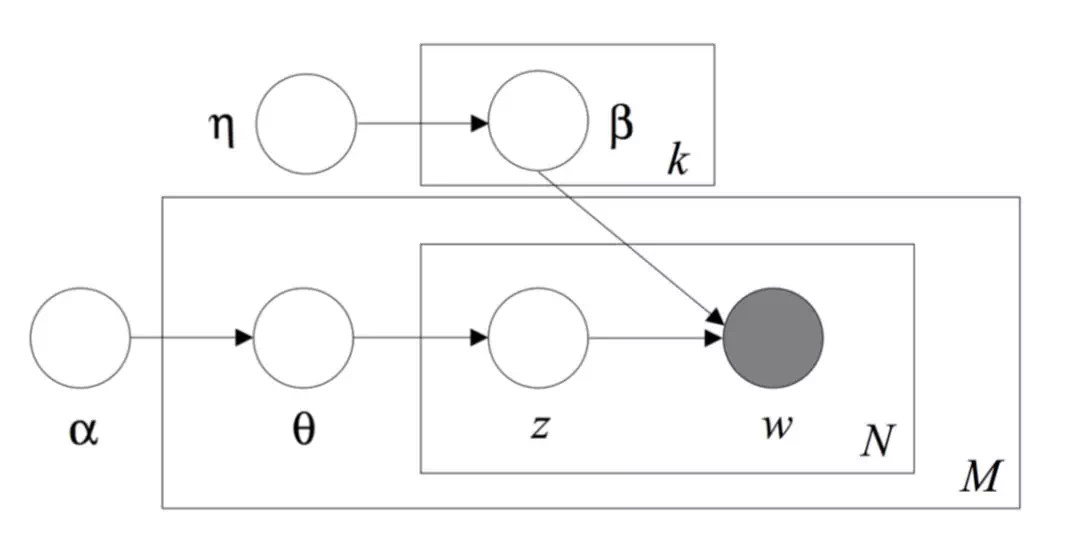
\includegraphics[width = 15cm]{lda.png}
\caption{The caption of this figure.}
\label{fig:figure1label}
\end{figure}


In the LDA model, a document is generated as follows:
\begin{enumerate}
  \item Sampling from Dirichlet distribution $\alpha$ to generate the topic $\theta$ distribution of document $i$.

  \item Sample the $j$th word of the topic $z_{i,j}$  of the document $i$ from the polynomial distribution of topics $\theta_i$.

  \item Sampling from Dirichlet distribution $eta$ to generate word distribution$\beta_{z_{i,j}}$ corresponding to topics$z_{i,j}$.

  \item Sampling from the polynomial distribution$\beta_{z_{i,j}}$  of words to finally generate words $w_{i,j}$.

\end{enumerate}

This probability map can be decomposed into two parts:
\begin{enumerate}
  \item $$\alpha \rightarrow \theta  \rightarrow z $$
This process means that when generating the m-th document, a candidate for a topical toll is generated, and then the topic of each word in the document is randomly generated according to the toll
  \item $$\eta \rightarrow \beta  \rightarrow w|k $$This process means that the word of the document is generated when the topic number is known, and the vector with the topic k is selected in the topic-word matrix, and then the word is generated according to this vector
\end{enumerate}

In the process of document construction,$ M$ documents correspond to $M$ independent Multinomial-Dirichlet conjugate structures, and $K$ topics also correspond to $K$ independent Multinomial-Dirichle conjugate structures. Among them, $M+K$ conjugate structures are all independent. Let’s discuss the document generative process further.


From the first decomposition,We know that $\alpha \rightarrow \theta$ represents the theme corresponding to all documents, which is subject to the Dirichlet distribution. And $\theta  \rightarrow z$  is to generate the theme corresponding to each word, subject to the multinomial distribution. and the Dirichlet distribution is the conjugate distribution of the polynomial distribution. All the whole is a conjugate structure
\begin{eqnarray*}
  f(z_k|\alpha) &=& \int f(z_k|p)f(p|\alpha) d_p \\
              &=& \int \prod_{k=1}^K p_k^{n_k} Dir(p|\alphha) d_p \\
              &=& \int \prod_{k=1}^K p_k^{n_k} \frac{1}{B(\alpha)}\prod_{k=1}^{K}p_k^{\alpha_k-1} d_p \\
              &=& \frac{1}{B(\alpha)}\int \prod_{k=1}{V}p_k^{n_k+\alpha_k-1} d_p \\
              &=& \frac{B(n_k+\alpha_k)}{B(\alpha)}
\end{eqnarray*}
Vector $n = (n_1,_2,..n_K)$ represents the number of words of topic $V$ in each document.
$B$ is the gamma function:
\[
  B(\alpha) = \frac{\prod_{i=1}^V\Gamma(\alpha_i)}{\Gamma(\sum_{i=1}^V \alpha_i)}
\]

For the second decomposition,We know that $\eta \rightarrow \beta$ represents the word-distribution corresponding to all topics, which is subject to the Dirichlet distribution. And $\beta  \rightarrow w|k $  is to generate the word corresponding to each topic, subject to the multinomial distribution. and the Dirichlet distribution is the conjugate distribution of the polynomial distribution. All the whole is a conjugate structure
\begin{eqnarray*}
  f(w|\beta) &=& \int f(w|\beta)f(\beta|\eta) d_{\beta} \\
              &=& \int \prod_{k=1}^V p_k^{n_k} Dir(p|\alpha) d_p \\
              &=& \int \prod_{k=1}^Vp_k^{n_k} \frac{1}{B(\alpha)}\prod_{k=1}^{V}p_k^{\alpha_k-1} d_p \\
              &=& \frac{1}{B(\alpha)}\int \prowd_{k=1}{V}p_k^{n_k+\alpha_k-1} d_p \\
              &=& \frac{B(n_k+\alpha_k)}{B(\alpha)}
\end{eqnarray*}
Vector $n = (n_1,_2,..n_V)$ represents the number of words generated by each topic $V$.

We assume two vector:
\[
  \vec{w} = (\vec{w_1},\vec{w_2},..\vec{w_k})
\]
\[
  \vec{z} = (\vec{z_1},\vec{z_2},..\vec{z_k})
\]


\begin{eqnarray*}
  p(\vec{w}\vec{z}|\alpha,\beta) & = & p(\vec{w}|\vec{z},\beta)p(\vev{z}|\alpha) \\
                                 & = & \prod_i^{K}\frac{B(\beta+n_k)}{\beta}\prod_i^M\frac{n_m+\alpha}{\alpha}
\end{eqnarray*}
$w_k$ indicates that these words were generated by the $k$th topic.

\subsection{Gibbs Sampling for LDA}
BY the joint probability distribution $p(\vec{w}\vec{z}|\alpha,\beta)$ in the previous subsection, we can use Gibbs Sampling to sample it.The $i$th word in the corpus  is denoted as $z_{i}$, where $i=(m,n)$ is a two-dimensional subscript, which corresponds to the $n$th word in the $m$ document. According to the Gibbs Sampling algorithm in the second subsection, we need to require the conditional distribution corresponding to any coordinate axis. Assuming the observed word $w_i=t$, then by Bayes' rule, we can easily get:
\begin{eqnarray*}
  p(z_i=k|\vec{z_{\neg_i}},\vec{w}) & \propto & p(z_i=k,w_i = t|\vec{z_{\neg_i}},\vec{w_{\neg_i}}) \\
  &=& \int p(z_i = k,w_i=t,\theta,\alpha|\vec{z_{\neg_i}},\vec{w_{\neg_i}})d_{\theta} d_{\alpha} \\
  &=& \int p(z_i=k,\theta|\vec{z_{\neg_i}},\vec{w_{\neg_i}}) p(w_i=t,\alpha|\vec{z_{\neg_i}},\vec{w_{\neg_i}})d_{\theta} d_{\alpha}\\
  &=&
\end{eqnarray*}

Finally, we get the Gibbs Sampling formula of the LDA model as:
\[
p(z_i=k|\vec{z_{\neg_i}},\vec{w}) \propto \frac{n_{m,\neg{i}}^{(k)}+\alpha_k}{\sum^K (n_{m,\neg{i})}+\alpha_k)} *
 \frac{n_{k,\neg{i}}^{(t)}+\beta_t}{\sum^V (n_{m,\neg{i})}+\beta_t)}
\]


The equation on the right can be seen as \[
  p(topic|doc)*p(word|topic)
\]


We summarize the LDA Gibbs sampling algorithm process. The first is the training process:
\begin{enumerate}
  \item  Choose the right number of topics 𝐾, choose the right hyperparameter vector 𝛼⃗$\vec{\alpha}$ and $\vec{\beta}$.
 \item Corresponding to each word of each document in the corpus, randomly assign a topic number $z$.
 \item Rescan the corpus, for each word, use Gibbs sampling formula to update its   topic
  \item number, and update the number of the word in the corpus.
Repeat the Gibbs sampling based on coordinate axis rotation in step 3 until the Gibbs sampling converges.
  \item Calculate the theme of each word in each document in the corpus, get the document theme distribution $\theta_d$, calculate the distribution of each theme in the corpus, get the LDA theme and word distribution $\beta_k$.
\end{enumerate}

\subsection{Perplexity and Inference}

In information theory, perplexity is a measure of judging the probability model or probability distribution prediction, and can be used to evaluate the quality of the model.
\[
  perplexity(D) = exp(-\frac{\sum_{k=1}^{M}p(\vec{w_k})}{\sum_{k=1}^{M}N_k})
\]
The denominator is the sum of all the words in the test set, that is, the total length of the test set. Where $p(\vec{w_k})$ refers to the probability of each word of document $k$ in the test set.
\begin{eqnarray*}
  p(\vec{w_k}) &=&\prod_{i=1}^{V}p(w_k^{(i)})\\
               &=&\prod_{i=1}^{V}\int p(w_k^{(i)}|z_i)p(z_i)d_{z_i}
\end{eqnarray*}

With the LDA model, for the new document doc, we only need to think that the topic-word matrix is stable and is provided by the model obtained from the training corpus, so we only need to estimate ttopic distribution of he document. The specific algorithm is as follows:
\begin{enumerate}
  \item  For each word $w_i$ in the current document, randomly initialize a topic number $z$.
  \item Use Gibbs Sampling formula to resample each word $w_i$.
  \item  Repeat the above process until Gibbs Sampling convergence.
  \item Statistics on the topic distribution in the document, the distribution is $\theta_i$.
\end{enumerate}

\section{Dirichlet belief networks}
As can be seen from the above, the bright distribution of topics and word matrices obey Dirichlet distribution, which is an effective assumption, but it also brings many limitations. Recently,people introduce different generative models
\subsection{Research on Topic Distribution}

The LDA model assumes that the topics are independent of each other, however, this assumption
It is very inconsistent with the actual data set. To overcome this defect, Blei
In 2006, a related topic model (Correlated Topic Model,
CTM)\cite{A CORRELATED TOPIC MODEL OF SCIENCE 1}, the model extracts the topic from the Logistic Normal distribution, overcoming the disadvantage that
 LDA model cannot extract relatation of  information between texts.This model mentioned
above have been successfully applied in extracting scientific subjects and image extraction.

Another well-known research on topic-distribution is Hierarchical Dirichlet processes\cite{Teh}.
Based on the deformation of Dirichlet Process,
HDP is A non-parametric Bayesian model that can automatically train the most suitable from the document set
Appropriate number of topics K. Nonparametric characteristics of HDP through Dirichlet process
Solve the problem of selecting the number of topics in LDA, and the experiment confirms  that
The optimal number of topics selected by HDP is equal to the optimal number of topics selected based on perplexity
.
LDA model assumes that topic of each word is subject to multinomial distribution and the document is converted into count  matrix by Bag of Word model.Poisson Factor \cite{Beta-Negative Binomial Process and Poisson Factor Analysis} Analysis introduces poisson distribution.
\[
  x_pi = \sum_{k=1}^{K} x_{pik}
\]
\[
  x_{pik} \sim Pois(\gamma_{pk}\theta_{ki})
\]
and topic-distribution is subject to gamma distribution:
\[
  \theta_{ki} \sim Gamma(r_k,\frac{p_k}{1-p_k})
\]

\subsection{Introduction of DIRBN}
Compared to considerable researchs  topic model,The word model has not been fully studied and The Dirichlet Belief Network (DBN)\cite{Zhao} introduces a deep generative model where each layer is weighted by sets of  topics.

Different from single layer dirichlet,DirBN model proposed a multi-layer Dirchlet layer generative process on word-distribution.The latent distri-
butions in each layer of DBN are generated as Dirichlet
random variables and can thus be interpreted as categorical
distributions.Then  the hidden units are connected with gamma-distributed weights.

In comparison to existing deep generative models,DirBN have better Interpretability on topics annd higher modelling accuracy.However,the current formulation of DBN odel suffers from decay during information passing.

DBN’s deep architecture is currently limited to
only a few layers. In order to obtain efficient Gibbs sam-
pling, DBN back-propagates the observed information from
the output layer to each hidden layer. The cost of the in-
formation back-propagation is that the information would
decay in a O(log) rate on passing through one layer to its
upper layer \cite{Zhou}. Therefore, little informa-
tion might be available after a few layer back-propagations

%%%%%%%%%%%%%
\chapter{Conclusion}\label{ccl}

In mathematics, certain kinds of mistaken proof are often exhibited, and sometimes collected, as illustrations of a concept of mathematical fallacy. There is a distinction between a simple mistake and a mathematical fallacy in a proof: a mistake in a proof leads to an invalid proof just in the same way, but in the best-known examples of mathematical fallacies, there is some concealment in the presentation of the proof. For example, the reason validity fails may be a division by zero that is hidden by algebraic notation. There is a striking quality of the mathematical fallacy: as typically presented, it leads not only to an absurd result, but does so in a crafty or clever way. Therefore these fallacies, for pedagogic reasons, usually take the form of spurious proofs of obvious contradictions. Although the proofs are flawed, the errors, usually by design, are comparatively subtle, or designed to show that certain steps are conditional, and should not be applied in the cases that are the exceptions to the rules. \\

\noindent The traditional way of presenting a mathematical fallacy is to give an invalid step of deduction mixed in with valid steps, so that the meaning of fallacy is here slightly different from the logical fallacy. The latter applies normally to a form of argument that is not a genuine rule of logic, where the problematic mathematical step is typically a correct rule applied with a tacit wrong assumption. Beyond pedagogy, the resolution of a fallacy can lead to deeper insights into a subject (such as the introduction of Pasch's axiom of Euclidean geometry and the five color theorem of graph theory). Pseudaria, an ancient lost book of false proofs, is attributed to Euclid. \\

\noindent Mathematical fallacies exist in many branches of mathematics. In elementary algebra, typical examples may involve a step where division by zero is performed, where a root is incorrectly extracted or, more generally, where different values of a multiple valued function are equated. Well-known fallacies also exist in elementary Euclidean geometry and calculus.

%%%%%%%%%%%%%%%%%%%%%%%%%%%%%%%%%%%%%%%%%%%%%%%%%%%%%%%%%%%%%%%%%%%%%%%%%%
\clearpage
\addcontentsline{toc}{chapter}{References}
\bibliographystyle{unswthesis}
\begin{thebibliography}{999}

\bibitem
{intro-back}
Blei, David M. "Probabilistic topic models." Communications of the ACM 55.4 (2012): 77-84.

\bibitem
{TEST}
Barron, K., Kung, E. and Proserpio, D., 2018, June. The Sharing Economy and Housing Affordability: Evidence from Airbnb. In EC (p. 5).

\bibitem
{BBG} Benzinger, H., Berkson, E. and Gillespie, T.A.,
Spectral families of projections, semigroups, and differential operators,
\textit{Tran. Amer. Math. Soc.} \textbf{275} (1983), 431--475.

\bibitem
{BG Fourier} Berkson, E. and Gillespie, T.A.,
Fourier series criteria for operator decomposability,
\textit{Integral Equations Operator Theory} \textbf{9} (1986), 767--789.

\bibitem
{BG Spectral} Berkson, E., and Gillespie, T.A.,
Spectral decompositions and harmonic analysis on UMD spaces,
\textit{Studia Mathematica} \textbf{112}(1) (1994), 12--49.

\bibitem
{BGM} Berkson, E. Gillespie, T.A. and Muhly, P.S.,
Abstract spectral decompositions guaranteed by the Hilbert transform,
\textit{Proc. London Math. Soc. (3)} \textbf{53} (1986), 489--517.

\bibitem
{Bourgain telaviv}
Bourgain, J., {\em Martingale transforms and geometry of Banach spaces},
Israel seminar on geometrical aspects of functional analysis
(1983/84), XIV, 16 pp., Tel Aviv Univ., Tel Aviv, 1984.

\bibitem
{Bourgain} Bourgain, J.,
Some remarks on Banach spaces in which martingale difference sequences are
unconditional,
\textit{Ark. Mat.} \textbf{21} (1983), 163--168.

\bibitem
{Bourg} Bourgain, J.,
Vector-valued singular integrals and the $H^1$-BMO duality,
\textit{Probability Theory and Harmonic Analysis} (ed. Chao, J. A.) (1986),
1--19.

\bibitem
{Burk3} Burkholder, D.L.,
A geometrical characterisation of Banach spaces in which martingale difference
sequences are unconditional,
\textit{Ann. Probability} \textbf{9} (1981), 997--1011.

\bibitem
{Burk2} Burkholder, D.L.,
A geometric condition that implies the existence of certain singular integrals
of Banach-space valued functions,
\textit{Proceedings of Conference on Harmonic Analysis in Honor of Antoni
Zygmund} (Chicago, Illinois, 1981), Wadsworth Publishers: Belmont,
1983, pp. 270--286.

\bibitem
{Burk4} Burkholder, D.L.,
Martingales and Fourier analysis in Banach spaces,
\textit{Lecture Notes in Mathematics} \textbf{1206} (1986), 61--108.

\bibitem
{Burk1} Burkholder, D.L.,
Martingale transforms,
\textit{Ann. Math. Statist.} \textbf{37} (1966), 1494--1504.

\bibitem
{Coifman} Coifman R.R., and Weiss, G.,
\textit{Transference methods in analysis},
Regional Conference Series in Mathematics 31,
Amer. Math. Soc., Providence, R.I., 1977.

\bibitem
{Con} Conway, J.,
\textit{A Course in Functional Analysis},
Springer-Verlag: New York, 1985.

\bibitem
{Dowson} Dowson, H.,
\textit{Spectral theory of linear operators},
London Math. Soc. Monographs, No. 12. Academic Press: New York, 1978.

\bibitem
{Doust}
Doust, I., Norms of $0$-$1$ matrices in $\CC_p$,  pp 50-55, Proc.
Centre Math. Appl. Austral. Nat. Univ., 39, Austral. Nat. Univ.,
Canberra, 2000.

\bibitem
{DG} Doust, I.  and Gillespie, T. A.,
Schur multipliers on $\CC_p$ spaces,
in preparation.

\bibitem
{Dun} Dunford, N., and Schwartz, J.T.
\textit{Linear operators I: General theory},
Pure and Applied Mathematics 7. Interscience: New York, 1958.

\bibitem
{Gaudry} Edwards, R.E., and Gaudry, G.I.,
\textit{Littlewood--Paley and Multiplier Theory},
Springer-Verlag: Berlin, 1977.

\bibitem
{Katznelson}
Katznelson, Y.,
\textit{An introduction to harmonic analysis},
Second corrected edition, Dover: New York, 1976.

\bibitem
{Gohberg}
Gohberg, I.C., and Kre\u{\i}n, M. G.,
\textit{Introduction to the theory of linear nonselfadjoint operators},
Translations of Mathematical Monographs, Vol. 18, Amer. Math. Soc.,
Providence, R.I., 1969.

\bibitem
{Gowers} Gowers, W. T., and Maurey, B.,
The unconditional basic sequence problem,
\textit{J. Amer. Math. Soc.} \textbf{6} (1993), 851--874.

\bibitem
{Lind}
Lindenstrauss, J., and Tzafriri, L.,
\textit{Classical Banach Spaces I and II},
Springer: Berlin, 1996.

\bibitem
{Pedersen}
Pedersen, G. K.,
\textit{Analysis Now},
Springer: New York, 1989.

\bibitem
{Stein1}
Stein, E. M.,
The development of square functions in the work of A. Zygmund,
\textit{Bulletin (New Series) of the Amer. Math. Soc},
\textbf{6} (1982), 5--30.

\bibitem
{Stein}
Stein, E. M.,
\textit{Topics in Harmonic Analysis Related to the Littlewood--Paley Theory},
Princeton UP: Princeton, 1970.
\end{thebibliography}

\end{document}
